\documentclass[tikz,border=1pt]{standalone}
\usepackage{tikz}
\usepackage{amsmath}
\usetikzlibrary{trees,positioning}
\begin{document}
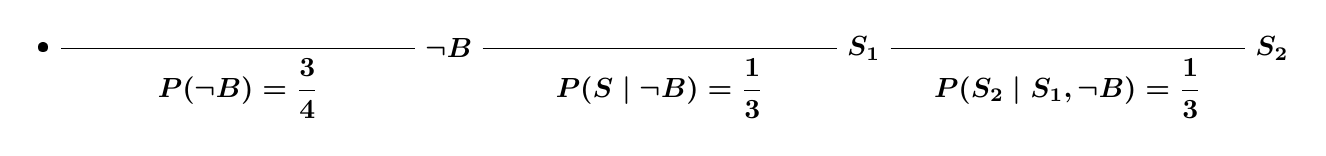
\begin{tikzpicture}[
    node distance=45mm,
    edge from parent/.style={draw, -, very thick},
    every node/.style={thick}
]
    \boldmath
    \node (start) {\textbullet};
    \node[right=of start] (not_b) {$\lnot B$};
    \node[right=of not_b] (S1) {$S_1$};
    \node[right=of S1] (S2) {$S_2$};

    \draw (start) -- (not_b) node[midway, below] {$P(\lnot B)=\dfrac{3}{4}$};
    \draw (not_b) -- (S1) node[midway, below] {$P(S\mid\lnot B)=\dfrac{1}{3}$};
    \draw (S1) -- (S2) node[midway, below] {$P(S_2\mid S_1,\lnot B)=\dfrac{1}{3}$};
\end{tikzpicture}
\end{document}